\section{Current State}

\subsection{Hardware}

The commissioning cluster runs in the antu nodes, with a capacity of 832 cores and 3.2TB of Ram. Details of its hardware configuration can be found in \href{https://ittn-014.lsst.io/}{ITTN-014 Computing Infrastructure}

\begin{figure}
    \centering
    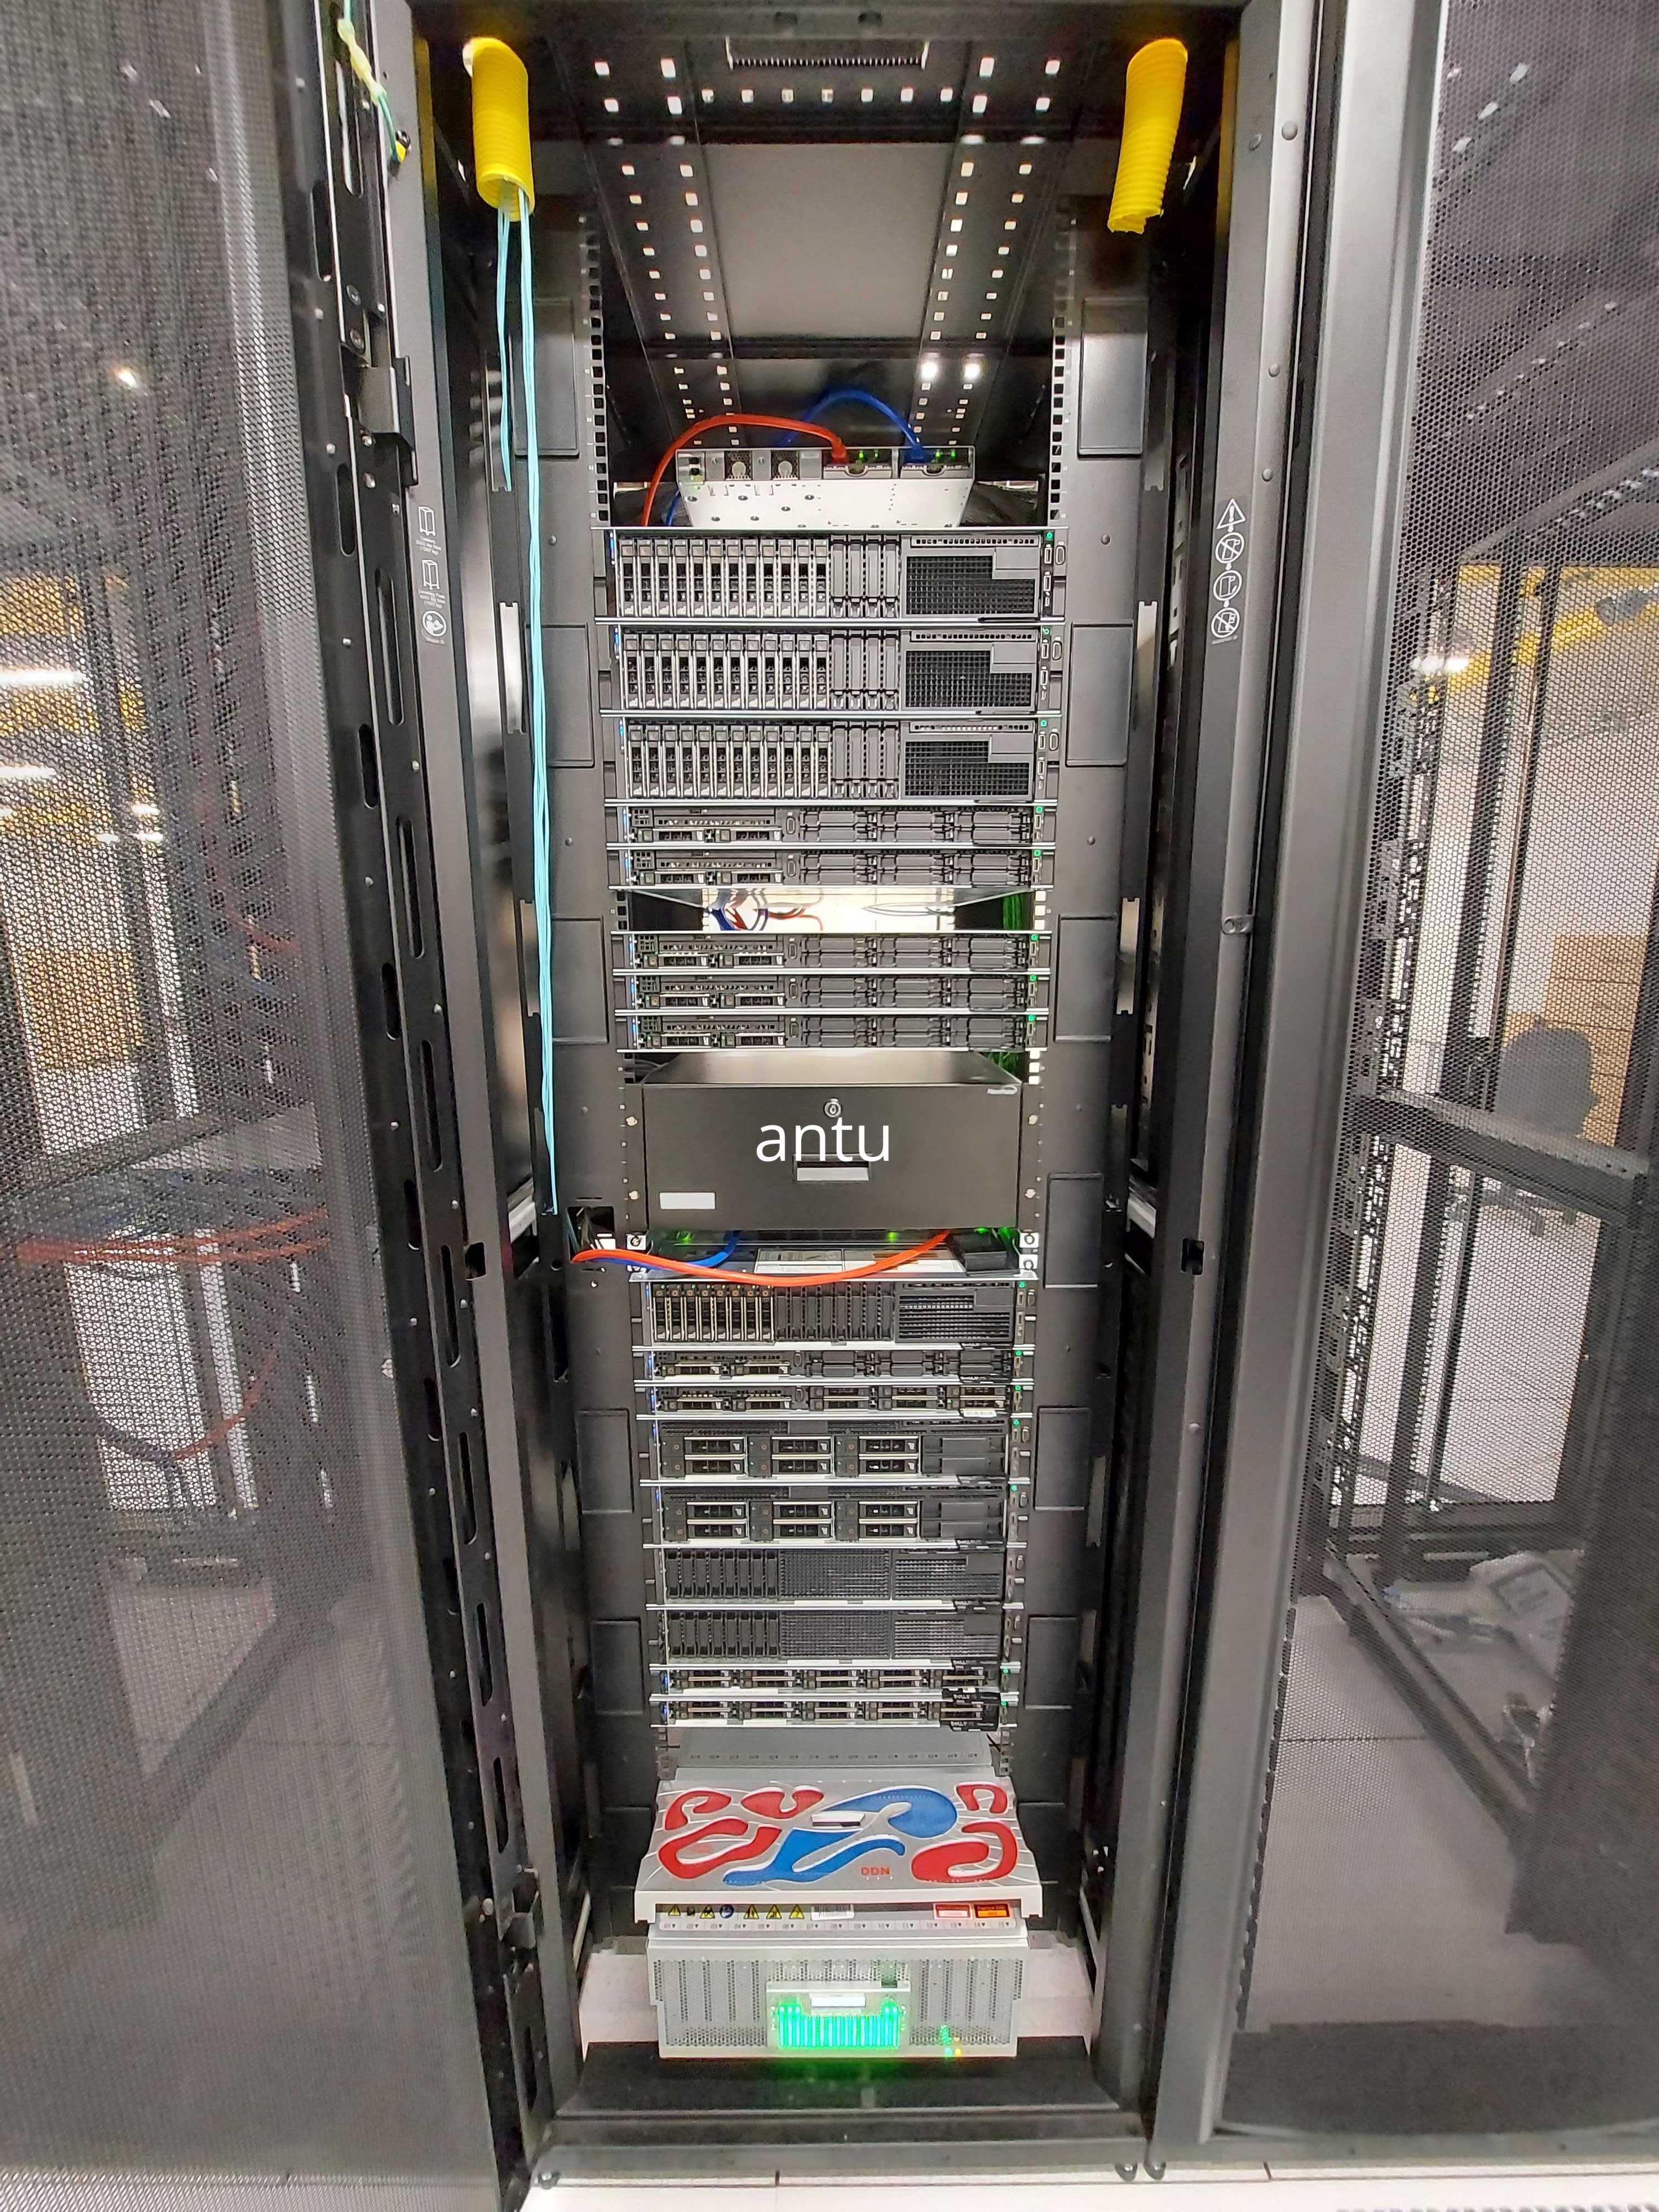
\includegraphics[width=10cm]{images/antu.jpg}
    \caption{antu cluster}
\end{figure}

The servers composing the antu cluster are a mix of different Dell models, previously deployed as forwarders and DTNs by NCSA. There's also a DDN unit of about 700TB of storage, and it is currently providing NFS mounts for Nublado
\newpage

The computing cluster at the summit is called yagan. It has a capacity of 576 cores and 2.2TB of Ram. 

\begin{figure}
    \centering
    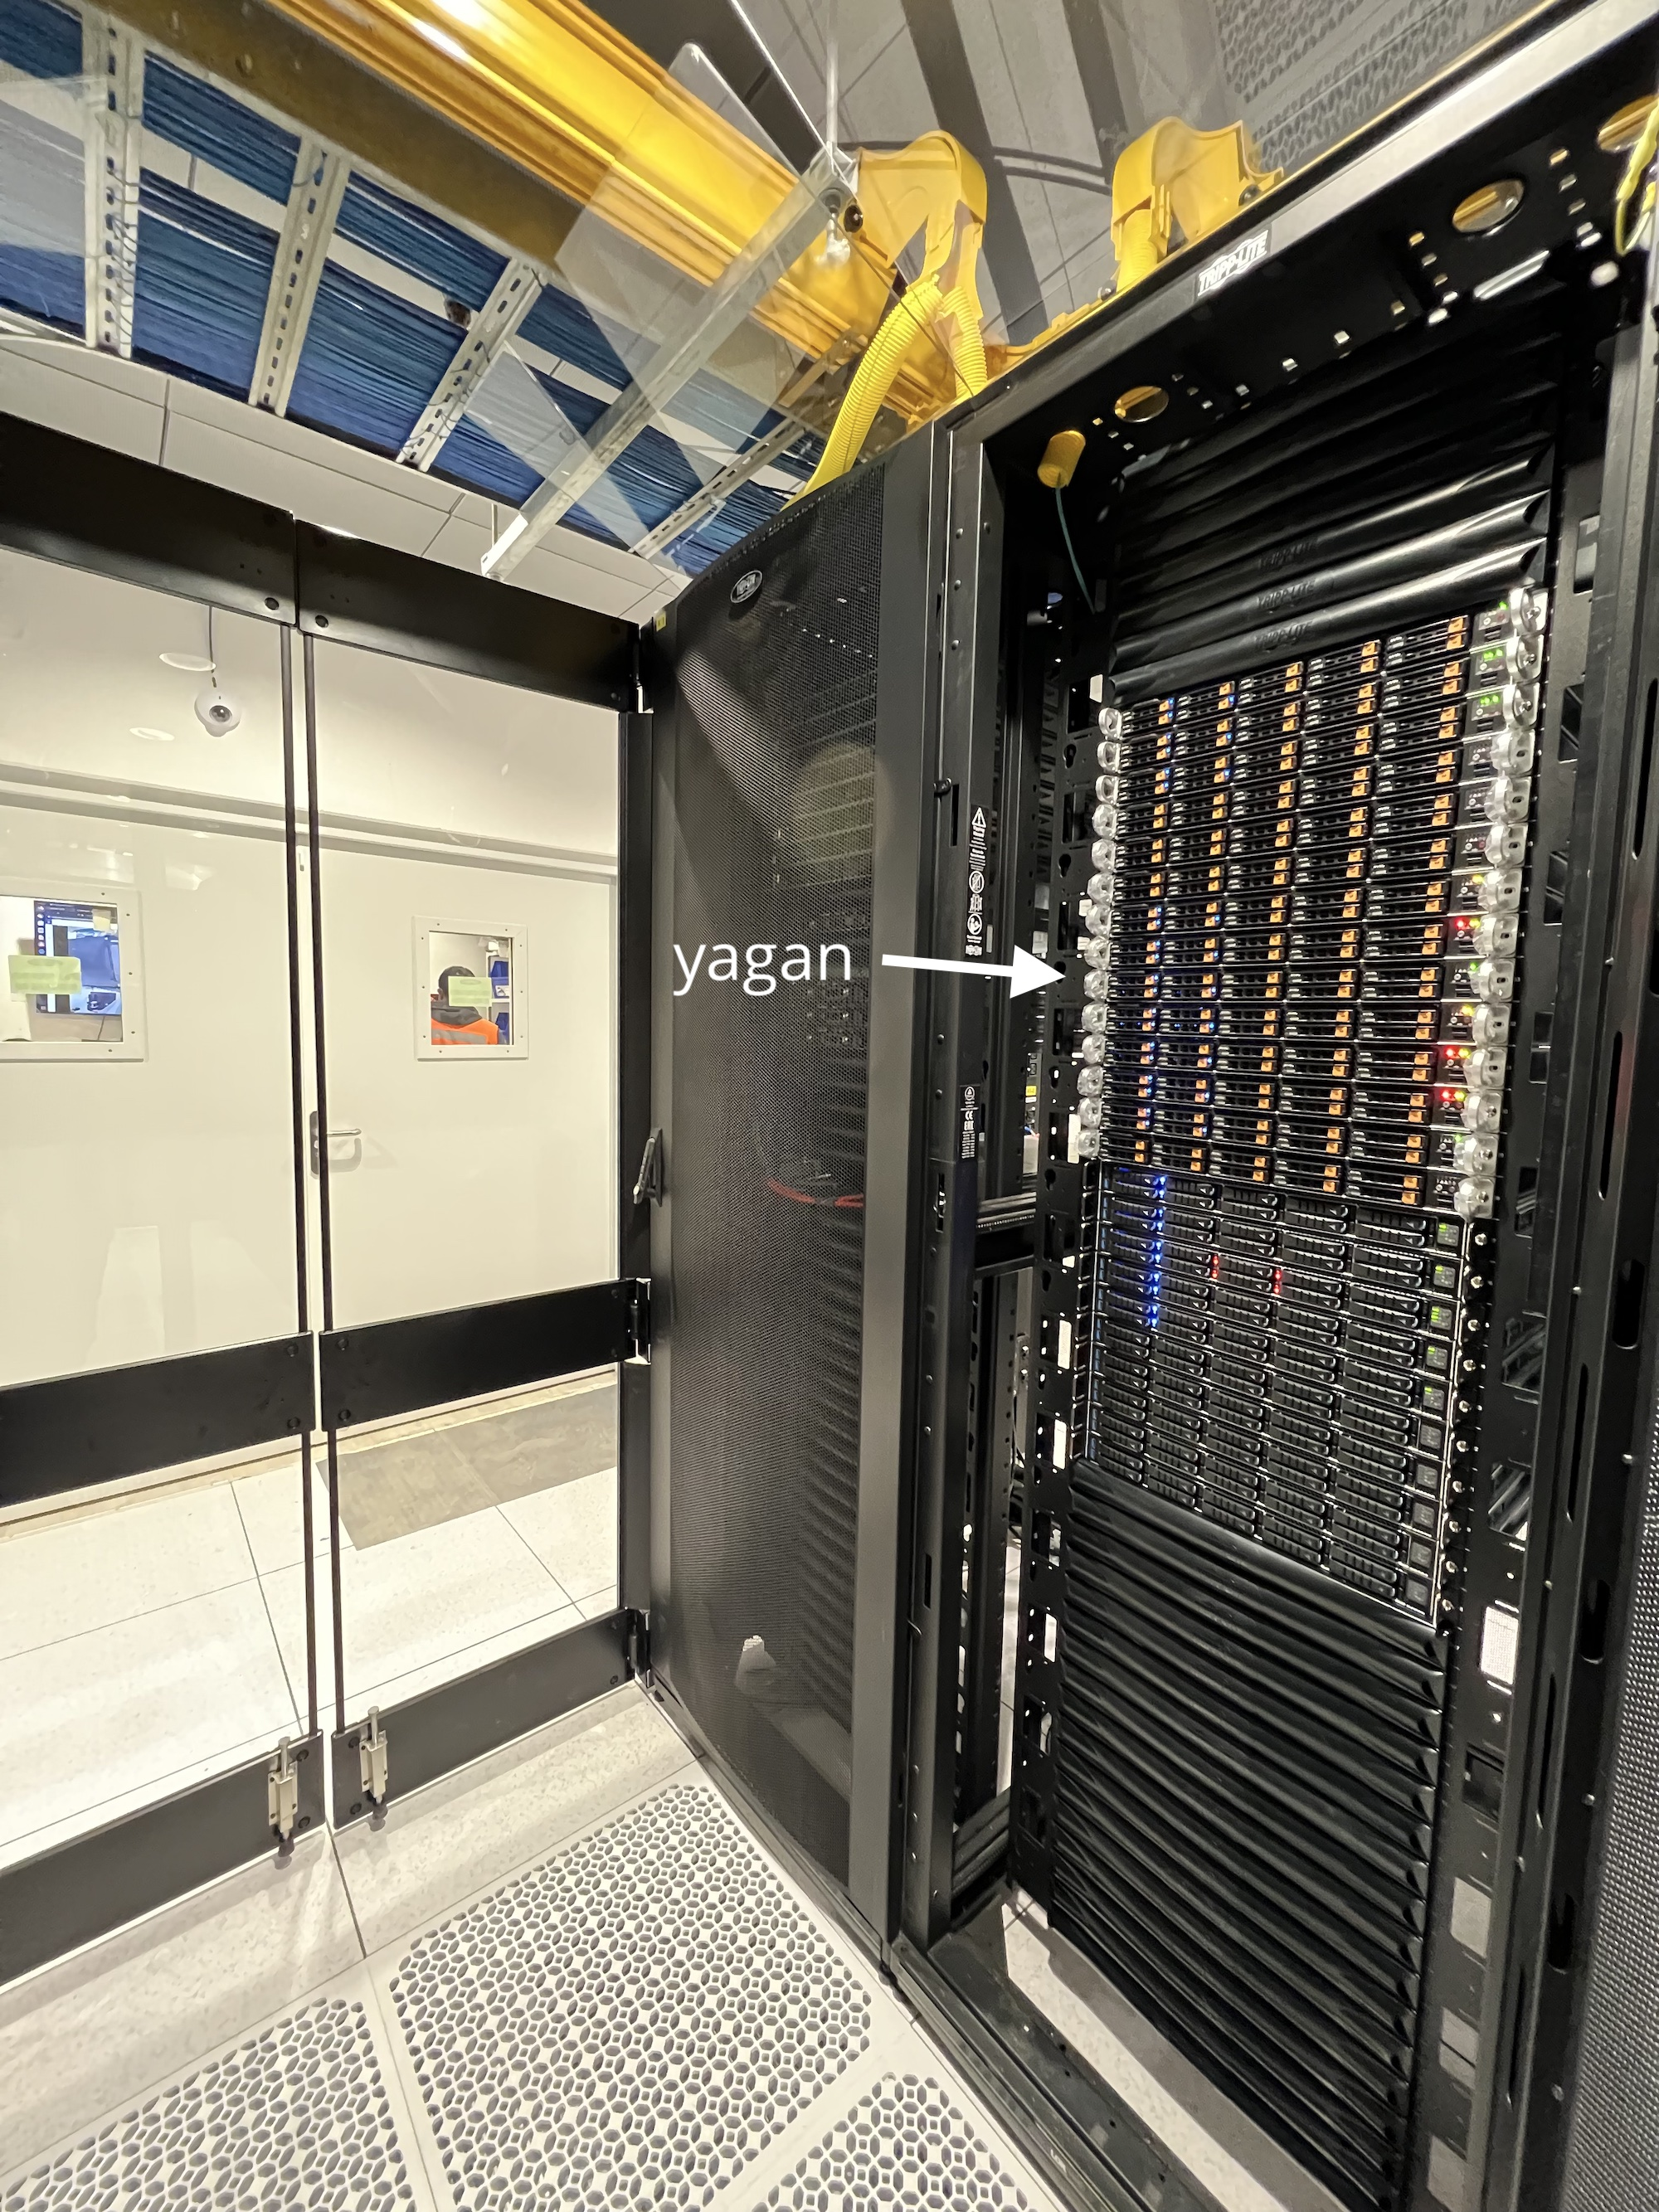
\includegraphics[width=10cm]{images/yagan.jpg}
    \caption{clusters at the summit}
\end{figure}

The servers in the yagan cluster have the same model and specs. This hardware model is shared with several other services and clusters at the summit, so they all work as a big pool of spares in case a node fails.  

\newpage

\subsection{Software}

All clusters are provisioned using  Rubin Devops Stack (puppet, ipa, etc)

The antu cluster runs:
\begin{itemize}
    \item Nublado
\end{itemize}

The yagan cluster runs: 
\begin{itemize}
    \item Rubin Science Platform
    \item EFD (in migration process)
    \item EAS CSCs
    \item Auxtel CSCs
    \item Kafka Producers 
    \item MT CSCs
    \item RubinTV
\end{itemize}

Regardless of the several components running in yagan, its cpu usage stays below 10\% and the RAM usage is never above 5\%


\section{Planned State}

Each rack at the summit has a maximum of 48RU, 8RU are used by network equipment such as switches and fiber headers. Therefore each rack could potentially host 40 servers of 1RU each.

The kubernetes clusters at the summit are all of 1RU with 64 cores; hence each rack could deliver up to 2500 cores. However, given the current commissioning and summit cluster size, the maximum size of the new computing cluster would be 1400 cores. 

\section{Storage}

Storage plays a crucial role in commissioning a cluster. The storage system should be fast and reliable to ensure that data can be accessed quickly and without interruption.

Rubin DevOps team prefer to have a single storage endpoint at the summit, which can simplify management and maintenance of the storage system. This can also help ensure consistency across the cluster and make it easier to manage access control and permissions for different users and applications. However, it's important to ensure that the chosen storage solution can meet the performance and capacity requirements of the cluster as well as any security and compliance requirements. 

The storage endpoint of the summit will be the LFA, hence will host all the LSSTCam data, the data products, and all the systems needing disk space , so all of these components should be factored in when determining the total storage capacity required for the cluster.

The following is an estimation of storage sizing:

LSSTCam:

15MB/CCD * 200 CCD/exposure * 2 exposure/visit * 1000 visit/day (including calibs) * 30 days = ~180TB

Data products:

LSSTCam Size * 15 = ~ 2700TB (considering that images will be uncompressed)

EFD:

As per DM-28554: ~25TB

Total of usable disk space: 3000TB (~3PB) 